\input{../preamble.tex}

\SetDate[24/03/2025]

\begin{document}
\pagestyle{fancy}
\fancyhead[L]{Seconde 5}
\fancyhead[C]{\textbf{Calendriers julien et grégorien}}
\fancyhead[R]{\today}

\begin{multicols}{2}

La Terre complète son tour autour du Soleil en environ 365,2422 jours. 
Un calendrier ne peut donc pas contenir 365 jours tous les ans si celui-ci doit être synchronisé avec les saisons.

Si le calendrier contient moins de 365,2422 jours, il sera en avance.
S'il contient plus de 365,2422 jours, il sera en retard

\begin{center}
    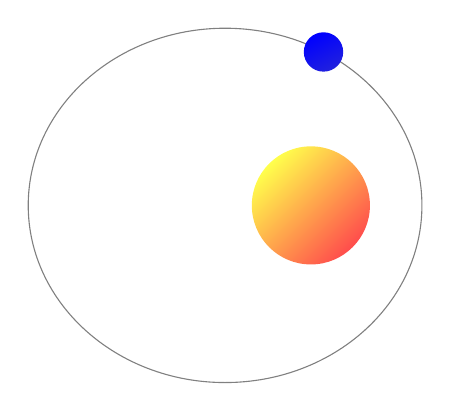
\begin{tikzpicture}[scale=2.5]
        \def\rS{0.3}                                % Sun radius

        \def\rE{0.1}                                % Earth radius
                                                    % Major radius of Earth's elliptical orbit = 1
        \def\eE{.9}                               % Excentricity of Earth's elliptical orbit       
        \pgfmathsetmacro\bE{.9}        % Minor radius of Earth's elliptical orbit  
          
        % This function computes the direction in which light hits the Earth.
        \pgfmathdeclarefunction{f}{1}{%
            \pgfmathparse{
                ((-\eE+cos(#1))<0) * ( 180 + atan( \bE*sin(#1)/(-\eE+cos(#1)) ) ) 
                +
                ((-\eE+cos(#1))>=0) * ( atan( \bE*sin(#1)/(-\eE+cos(#1)) ) ) 
            }
        }

        % This function computes the distance between Earth and the Sun,
        % which is used to calculate the varying radiation intensity on Earth.
        \pgfmathdeclarefunction{d}{1}{%
            \pgfmathparse{ sqrt((-\eE+cos(#1))*(-\eE+cos(#1))+\bE*sin(#1)*\bE*sin(#1)) }
        }

        % Draw the elliptical path of the Earth.
        \draw[thin,color=gray] (0,0) ellipse (1 and \bE);

        % Draw the Sun at the right-hand-side focus
        \shade[
            top color=yellow!70,
            bottom color=red!70,
            shading angle={45},
            ] ({sqrt(1-\bE*\bE)},0) circle (\rS);
         %\draw ({sqrt(1-\b*\b)},-\rS) node[below] {Sun};

        % Produces a series of frames showing one revolution
        % (the total number of frames is controlled by macro \N)
        \pgfmathtruncatemacro{\N}{12}
        \foreach \k in {2}{
            \pgfmathsetmacro{\Earthangle}{360*\k/\N}
            \pgfmathsetmacro{\Moonangle}{3*360*\k/\N} % <--- change the multiplying factor to suit your needs
            % Draw the Earth at \Earthangle
            \pgfmathsetmacro{\radiation}{100*(1-\eE)/(d(\Earthangle)*d(\Earthangle))}
            \colorlet{Earthlight}{yellow!\radiation!blue}
            \pgfmathparse{int(\k+1)}
                \shade[
                    top color=Earthlight,
                    bottom color=blue,
                    shading angle={90+f(\Earthangle)},
                    ] ({cos(\Earthangle)},{\bE*sin(\Earthangle)}) circle (\rE);
                 %\draw ({cos(\Earthangle)},{\bE*sin(\Earthangle)-\rE}) node[below] {Earth};  

        }
    \end{tikzpicture}
\end{center}

\end{multicols}



\subsection*{Calendrier julien\footnote{De Jules César (né en 100 av. J.-C., mort en 44 av. J.-C.).}}

En $46$ av. J.-C., Jules César introduit la règle de l'année bissextile.

\exe{}{
	\begin{enumerate}
		\item
		Trouver un entier naturel $a \in \N$ non nul tel que
			\[ 365{,}2422 \approx 365 + \dfrac1a.\]

		\item
		En déduire la règle d'année bissextile du calendrier julien.
		
		\item
		Au bout de 1 600 ans, de combien de jours le calendrier est-il en retard ?
	\end{enumerate}
}{exe:1}{}

\subsection*{Calendrier grégorien\footnote{Du pape Grégoire XIII (1502-1585).}}

En 1582, plus de 1 600 ans après l'introduction de la règle d'année bissextile, le calendrier julien prend donc un retard notoire.
Le pape Grégoire XIII promulgue alors une réforme du calendrier, ainsi créant le calendrier grégorien encore utilisé aujourd'hui.

Afin de corriger le problème de dérive du calendrier, une nouvelle règle est ajoutée à la définition d'année bissextile.

\exe{}{
	\begin{enumerate}
		\item
		Trouver un entier naturel $b \in \N$ tel que
			\[ 365{,}2422 \approx 365 + \dfrac14 - \dfrac{b}{400}.\]

		\item
		En déduire la règle d'année bissextile du calendrier grégorien.
		
		\item
		Au bout de combien d'années le calendrier est-il en retard d'un jour ?
	\end{enumerate}
}{exe:2}{}

\subsection*{Un nouveau calendrier ?}

\exe{}{
	\begin{enumerate}
		\item
		Trouver un entier naturel $c \in \N$ tel que
			\[ 365{,}2422 \approx 365 + \dfrac14 - \dfrac{3}{400} - \dfrac{c}{4000}.\]

		\item 
		Créer une nouvelle règle d'année bissextile.
		\item
		Calculer le nombre d'années avant que votre calendrier soit en retard d'un jour.
	\end{enumerate}
}{exe:3}{}

%%%%%%%%%%%

\newpage
\fancyhead[C]{\textbf{Solutions}}
\shipoutAnswer

\end{document}